

% 往 inference time 上靠

\section{Analysis}

\subsection{Retrieval Efficiency}
% To show the efficiency of our methods, we compare the average retrieve counts over the test samples on 2WikiMultihopQA and HotpotQA. 
% As shown in Table~\ref{tab:efficiency}, DRAGIN的检索次数受到阈值和不同数据集的影响很大,特别的对于不同的数据需要不同的阈值,as we know 2WikiMultihopQA的数据需要的evidence比 hotpotqa包含的数据需要的evidence要多一些,由于它有更多复杂的多跳问题,然后,对比相同的threshold,hotpotqa调用检索的次数却比2wiki的多,which展现了它的不鲁棒性。
% 相反的,我们的方法普遍使用了较少次数的检索,同时检索的次数和query的难度相关度较大

% To demonstrate the efficiency of our methods, we compare the average retrieval counts across test samples on 2WikiMultihopQA and HotpotQA. 

% As shown in Table~\ref{tab:efficiency}, we statistics the retrieval counts and answer accuracy for both the DRAGIN baseline and our method.
% Our method achieves a great balance between effectiveness and efficiency.
% In contrast, the retrieval counts of DRAGIN are significantly influenced by the threshold and the specific dataset.
% Moreover, different datasets require different thresholds due to the complexity of their queries.
% For instance, 2WikiMultihopQA requires more evidence because it contains more complex multi-hop questions compared to HotpotQA.
% However, when DRAGIN uses the same threshold, HotpotQA requires more retrievals than 2WikiMultihopQA, highlighting DRAGIN's lack of robustness.
% Conversely, our method consistently uses fewer retrievals, and the number of retrievals is more closely related to the difficulty of the queries.



To demonstrate the efficiency of our method, we compare the average number of retrievals on 2WikiMultihopQA and WebQuestions. As shown in Table~\ref{tab:efficiency}, We have following observations:
% 我们主要有几个发现
% our method has two main advantages:
% 1. 我们的方法是效果最好的里用的最少的
% 2. confidence 方法在不同的数据集中使用相同的阈值展现出了非常不鲁棒性
% 3. auto rag总是需要大量的检索次数
1) DeepRAG can achieve higher accuracy with relatively lower retrieval costs, attributed to its dynamic usage of internal knowledge.
% 
2) Confidence-based approaches demonstrate limited robustness across datasets.  
For instance, both FLARE and DRAGIN methods doesn't trigger retrieval under the default confidence threshold in WQ.
% For instance, while using identical thresholds, both FLARE and DRAGIN methods show inconsistent behavior: they trigger approximately one retrieval per query in 2WMQA, but fail to reach the retrieval threshold entirely in WQ. This inconsistency highlights the challenge of maintaining reliable performance across different datasets using confidence-based methods.
% 
3) Iterative retrieval-based approaches typically require numerous retrieval operations.
% 
Therefore, efficient adaptive retrieval methods like DeepRAG become crucial for optimizing resource utilization while maintaining performance.

% TODO
\setlength{\tabcolsep}{3pt}
\begin{table}
\centering
\caption{Efficiency of Different Methods}
\vspace{-0.1in}
\label{tab:efficiency}
% \resizebox{\textwidth}{!}{%
\scalebox{0.65}{%
\begin{tabular}{|c|ccc|ccc|ccc|}
  \hline
  \multirow{2}{*}{} & \multicolumn{3}{c|}{\textbf{memory size (MB)}} & \multicolumn{3}{c|}{\textbf{training time (s)}} & \multicolumn{3}{c|}{\textbf{matching time (s)}}\\
  % \cline{2-7}
  % {} & MByte & seconds/ep & seconds\\
  {} & \textbf{Beijing} & \textbf{Porto} & \textbf{Chengdu} & \textbf{Beijing} & \textbf{Porto} & \textbf{Chengdu} & \textbf{Beijing} & \textbf{Porto} & \textbf{Chengdu}\\
  % \cline{2-7}
  % {} & (MByte) & (minutes/ep) & (seconds/K) & (MByte) & (minutes/ep) & (seconds/K)\\
  \hline
  \textbf{MDP} & 1819MB & 2039MB & 2122MB & - & - & - & 389.14s & 361.15s & 599.51s  \\
  \textbf{HMM} & 1209MB & 1388MB & 1361MB & - & - & - & 427.97s & 380.05s & 589.08s \\
  % \hline
  \textbf{FMM} & 897MB & 931MB & 981MB & - & - & - & 1.13s & 1.02s & 1.87s \\
  % \hline
  \textbf{AMM} & 957MB & 1013MB & 1124MB & - & - & - & 3.42s & 3.05s & 5.16s \\
  % \hline
  \textbf{MTrajRec} & 9045MB & 12428MB & 11265MB & 182.4s & 2200.2s & 25672.4s & 51.22s & 42.27s & 73.68s\\
  % \hline
  \textbf{L2MM} & 9087MB & 11875MB & 10898MB & 189.1s & 2314.2s & 27032.2s & 6.71s & 5.26s & 9.10s\\
  % \hline
  \textbf{GraphMM} & 8537MB & 11752MB & 10378MB & 48.4s & 645.2s & 7311.4s & 8.06s & 6.96s & 11.18s\\
  % \hline
  \textbf{\modelName} & 2530MB & 2299MB & 2357MB & 11.9s & 126.4s & 1507.8s & 1.09s & 0.95s & 1.65s\\
  \hline
\end{tabular}}
\vspace{-0.15in}
\end{table}

% % Table generated by Excel2LaTeX from sheet 'Sheet2'
% \begin{table}[htbp]
%   \centering
%     \begin{tabular}{cccc}
%     \hline
%     Method & No-Ret Acc & Ret Acc & Overall Acc \\
%     \hline
%     FLARE & 0.004  & 0.986  & 0.495 \\
%     DRAGIN & 0.000  & 1.000  & 0.500  \\
%     UAR   & 0.401  & 0.896  & 0.648  \\
%     TAARE & 0.000  & 1.000  & 0.500  \\
%     Auto-RAG & 0.000  & 1.000  & 0.500  \\
%     DeepRAG-Imi & 0.656  & 0.762  & 0.709  \\
%     DeepRAG  & 0.730  & 0.756  & 0.743 \\
%     \hline
%     \end{tabular}%
%     \caption{Add caption}
%   \label{tab:addlabel}%
% \end{table}%



% Table generated by Excel2LaTeX from sheet 'Sheet2'
\begin{table}[htbp]
  \centering
  \resizebox{\linewidth}{!}{
    \begin{tabular}{ccccc}
    \toprule
    Method &  F1 &  Acc & Balanced Acc & MCC \\
    \midrule
    FLARE & 0.000  & 0.718  & 0.500  & 0.000 \\
    DRAGIN & 0.007  & 0.709  & 0.495  & -0.045  \\
    UAR   & 0.481  & \textbf{0.756}  & 0.648  & 0.341  \\
    TAARE & 0.127  & 0.712  & 0.518  & 0.078  \\
    % 0.12727272727272723 0.712 0.5184318141409352 0.07759714836703908
    Iter-DRAG & 0.000 & 0.718 & 0.500 & 0.000 \\
    Auto-RAG & 0.000 & 0.718 & 0.500 & 0.000  \\
    DeepRAG-Imi & 0.580  & 0.732  & 0.709  & 0.393  \\
    DeepRAG  & \textbf{0.621}  & 0.749  & \textbf{0.743}  & \textbf{0.451} \\
    \bottomrule
    \end{tabular}%
    }
    \caption{Analysis of internal knowledge utilization across different adaptive retrieval methods on 2WikiMultihopQA.}
\label{tab:relevance}%
\end{table}%




\subsection{Relevance to Parametric Knowledge}
% TODO 这里要讲的更清楚
In this section, we investigate the relationship between retrieval needs and internal knowledge to demonstrate how effectively \textit{atomic decisions} explores the knowledge boundary.
% 
The detail setting are shown in Appendix~\ref{relevance}.
We report four metrics. 
F1 score and Accuracy serve as basic performance measures, while balanced accuracy and Matthews Correlation Coefficient(MCC)~\cite{Wikipedia_PhiCoefficient} are employed to account for the class imbalance between retrieval-required and retrieval-not-required cases. 




% 1. DeepRAG 展现了很好的相关性 2. FLARE,DRAGIN,TAARE展现了较高的Acc 但是balancedacc和MCC并不高,因为他们的成功仅来源于成功检索的case,对于没有必要检索的case并没有正确规避
As shown in Table~\ref{tab:relevance}, we find that: 1) 
DeepRAG demonstrates superior relevance performance across F1, balanced accuracy, and MCC metrics.
This suggests that DeepRAG successfully identifies retrieval necessity by exploring knowledge boundary;
% 
2) While FLARE, DRAGIN, and TAARE exhibit high accuracy scores, their relatively low balanced accuracy and MCC scores suggest they mainly succeed in retrieval-required cases but struggle to properly avoid unnecessary retrievals.


\subsection{Different Inference Strategy}
% To gain a deep insight of the effectiveness of adaptive retrieval, 我们评估了DeepRAG在完全使用内部知识以及完全使用检索的表现。
% Specifically,对于all-internal setting, we force LLM to use internal knowledge to answer each subquery. For all-external setting, we force LLM to use external knowledge(retrieval) to answer each subquery.
% 如Figurexxx所示,depend solely on internal knowledge achieves 极低的效果,while depend solely on external knowledge achieves 相对高但巨大检索成本的结果。
% 和他们不同,DeepRAG通过自适应的选择内部知识or外部知识实现了great achievement on both internal and external knowlege.
% % 
% Specifically, 对于DeepRAG比all retrieve高,我们认为这是由于在部分场景下retrieval由于long context or unrelevant knowledge会让模型不那么faithful,反而不如使用内部知识。

To gain a deep insight into the effectiveness of \textit{retrieval narartive}, we evaluate DeepRAG's performance under two extreme scenarios: relying solely on internal knowledge and using retrieval in each subquery.
% 
% Specifically, for the all-internal setting, we force LLM to use internal knowledge to answer each subquery. For the all-external setting, we force LLM to use external knowledge to answer each subquery.
As shown in Figure~\ref{fig:analysis1}, depending solely on internal knowledge yields poor performance, while relying entirely on external knowledge achieves relatively higher accuracy but incurs substantial retrieval costs.
In contrast, DeepRAG achieves superior performance by adaptively selecting between internal and external knowledge sources.
% 
Specifically, DeepRAG outperforms the retrieve only approach. This may be attributed to the fact that in certain scenarios, retrieval can hinder model performance due to long context or irrelevant knowledge, making internal knowledge the more reliable choice.

\subsection{Question Decomposition Effectiveness}
% 训练/inference迭代数分布
% subquery中名词、代词统计
% \usepackage{xcolor}
% \usepackage{pgf-pie}

% We systematically analysis the effectiveness of question decompostion of DeepRAG.
% As shown in Figure~\ref{pie}, 我们统计了不同问题对应的subquery数量分布和检索次数分布。question多数在3-5轮,检索次数集中在0-2轮,这展现了,DeepRAG能过有效拆解问题,并且避免冗余检索。

We systematically analyze the effectiveness of question decomposition in \textit{retrieval narrative}. 
As shown in Figure~\ref{pie}, we present the distribution of subquery counts and retrieval attempts for different questions. Most questions require 3-5 decomposition steps, while retrieval attempts are primarily concentrated within 0-2 rounds. This demonstrates that DeepRAG effectively decomposes questions while minimizing redundant retrieval.

\begin{figure}[h]
    \centering
    \begin{minipage}[]{0.23\textwidth}
        \centering
        \scriptsize
        \begin{tikzpicture}
            \pie[text=legend, sum=1000, radius=1,
                color={soft1, soft2, soft3, soft4, soft5}]{
                683/3, 
                65/4, 
                61/5, 
                191/$\geq$6
            }
        \end{tikzpicture}
        \normalsize
        (a)
    \end{minipage}
    \hfill
    \begin{minipage}{0.23\textwidth}
        \centering
        \scriptsize
        \begin{tikzpicture}
            \pie[text=legend, sum=1000, radius=1, 
                color={soft1, soft2, soft3, soft4, soft5}]{
                381/0, 
                177/1, 
                433/2, 
                9/$\geq$3
            }
        \end{tikzpicture}
        \normalsize
        (b)
    \end{minipage}
    \caption{(a) Subquery Statistics. (b) Retrieval Statistics.}
    \label{pie}
\end{figure}


% Moreover, we 统计了subquery中的WH-words, nouns, verbs, and conjunctions  的平均 in Figure~\ref{tab:atomic}, which demonstrates that DeepRAG decompose atomic query with 更少的代词和连接词。

Moreover, we analyze the average counts of WH-words, nouns, verbs, and conjunctions in subqueries, as shown in Figure~\ref{fig:atomic}. The results indicate that DeepRAG decomposes atomic queries with fewer pronouns and conjunctions.

% %TODO 改成柱状图
% \begin{table}[htbp]
%   \centering
%     \begin{tabular}{lrrrr}
%     \toprule
%           & \multicolumn{1}{l}{WH} & \multicolumn{1}{l}{Noun} & \multicolumn{1}{l}{Verb} & \multicolumn{1}{l}{And/Or} \\
%           \midrule
%     DeepRAG & 0.98  & 0.04  & 1.13  & 0.12  \\
%     Auto-RAG & 1.26  & 0.30  & 2.05  & 0.77  \\
%     \bottomrule
%     \end{tabular}%
%     \caption{Average counts of WH-words, nouns, verbs, and conjunctions (and/or) per subquery.}
% \label{tab:atomic}%
% \end{table}%


\begin{figure}[htbp]
    \centering
    \begin{minipage}[b]{0.45\textwidth}
        \centering
        \resizebox{\textwidth}{!}{
            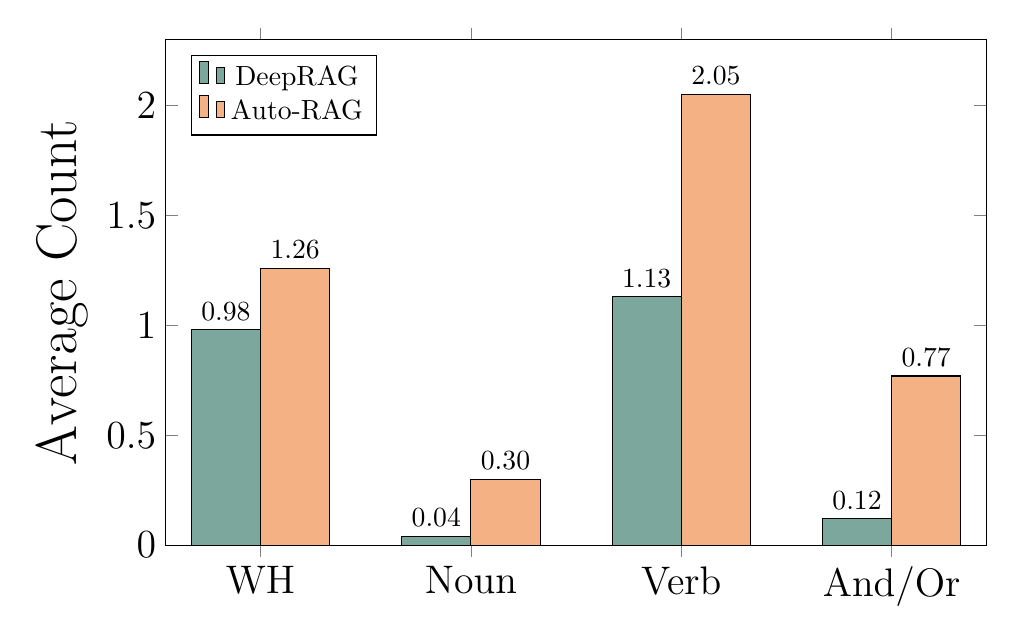
\begin{tikzpicture}
                \begin{axis}[
                    ybar=0pt,
                    width=12cm,
                    height=8cm,
                    bar width=25pt,
                    symbolic x coords={WH,Noun,Verb,And/Or},
                    xtick=data,
                    ymin=0,
                    ymax=2.3,
                    yticklabel style={font=\Large},
                    label style={font=\LARGE},
                    ylabel={Average Count},
                    ylabel style={font=\huge},
                    legend pos=north west,
                    nodes near coords style={/pgf/number format/.cd,fixed,fixed zerofill,precision=2},
                    nodes near coords,
                    % every node near coord/.append style={font=\Large, yshift=2pt},
                    enlarge x limits=0.15,
                    x tick label style={font=\Large},
                ]

                \addplot[
                    fill={rgb,255:red,123; green,167; blue,157},
                    bar shift=-12.5pt  % 手动调整第一组柱子位置
                ] coordinates {
                    (WH,0.98) (Noun,0.04) (Verb,1.13) (And/Or,0.12)
                };
                \addlegendentry{DeepRAG}

                \addplot[
                    fill={rgb,255:red,244; green,177; blue,131},
                    bar shift=12.5pt  % 手动调整第二组柱子位置
                ] coordinates {
                    (WH,1.26) (Noun,0.30) (Verb,2.05) (And/Or,0.77)
                };
                \addlegendentry{Auto-RAG}

                \end{axis}
            \end{tikzpicture}
        }
        \caption{Average counts of WH-words, nouns, verbs, and conjunctions (and/or) per subquery.}
        \label{fig:atomic}
    \end{minipage}
\end{figure}

\subsection{Ablation Study}
In this section, we conducted experiments to validate the effectiveness of DeepRAG's data construction and training process. 

% Firstly, we analyze the impact of different methods for selecting sythesied data on model performance.
% Specifically, 相比于默认的选择检索cost最少的路径,我们比较了两种不同的选择策略,一种是选择检索cost最多的路径训练,一种是随机选择路径训练。
% The ablation of Imitation Learning process is shown in Table~\ref{tab:sft-abla}, 
% 我们可以发现,DeepRAG-Imi可以让模型在模仿学习阶段就学会初步的探索知识边界。特别的,CAG在这一阶段表现较差是因为它是time-sensitive的,which always need retrieval the up-to-data information. Morever, in Figure2(a), 我们可以发现相比most-retrieve cost 和random方法,DeepRAG-Imi可以achieve更低检索开销和更高的平均性能。
% 
% Table generated by Excel2LaTeX from sheet 'abaltion'
% \begin{figure*}[htbp]
%     \centering
%     \begin{minipage}[b]{0.32\textwidth}
%         \centering
%         \includegraphics[width=\textwidth]{figure/analysis1.pdf}
%         \caption{Comparative analysis of retrieval strategies: all internal or external.}
%         \label{fig:analysis1}
%     \end{minipage}
%     \hfill
%     \begin{minipage}[b]{0.66\textwidth}
%         \centering
%         \begin{minipage}[b]{0.48\textwidth}
%             \centering
%             \includegraphics[width=\textwidth]{figure/ablation1.pdf}
%             (a)
%         \end{minipage}
%         \hfill
%         \begin{minipage}[b]{0.48\textwidth}
%             \centering
%             \includegraphics[width=\textwidth]{figure/ablation2.pdf}
%             (b)
%         \end{minipage}
%         \caption{Average score and retrievals on the ablation study for Imitation Learning and Chain of Calibration. }
%         \label{fig:ablation}
%     \end{minipage}
% \end{figure*}






\begin{figure*}[htbp]
    \centering
    \begin{minipage}[b]{0.32\textwidth}
        \centering
        % \includegraphics[width=\textwidth]{figure/analysis1.pdf}
            \resizebox{\textwidth}{!}{
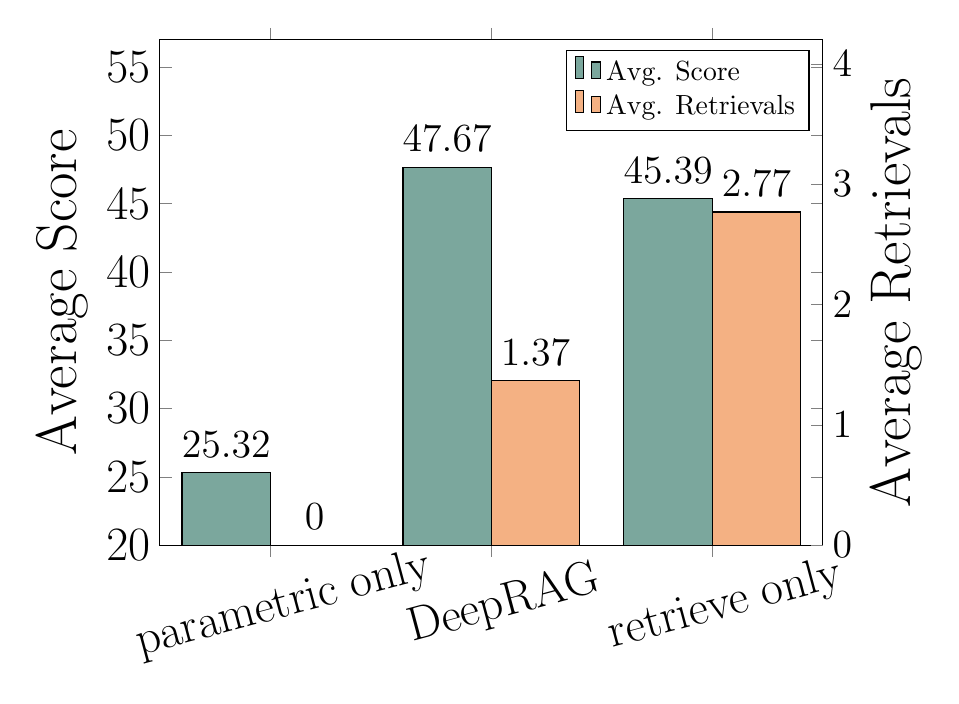
\begin{tikzpicture}

    %=======================%
    %   第一个 axis (左Y轴)
    %=======================%
    \begin{axis}[
        width=10cm,
        height=8cm,
        ybar,
        xmin=0.5, xmax=3.5,
        ymin=20, ymax=57,
        xtick={1,2,3},
        xticklabels={parametric only,DeepRAG,retrieve only},
        ticklabel style={font=\LARGE},
        xticklabel style={
            rotate=15,
            anchor=center,
            yshift=-18
        },
        label style={font=\Large},
        ylabel={Average Score},
        ylabel style={font=\huge},
        bar width=0.4,
        legend style={
            % at={(0.5,1.15)},    % 调整图例位置到图表上方
            anchor=north east,       % 设置锚点为北
            font=\normalsize,
            cells={anchor=west},
        },
    ]

    %------ 左柱: Avg. Score ------%
    % 3 个方法, x=1-0.2=0.8, 2-0.2=1.8, 3-0.2=2.8
    \addplot[
        fill={rgb,255:red,123; green,167; blue,157},
        nodes near coords,
        point meta=y,
        every node near coord/.append style={font=\Large, yshift=2pt}
    ] coordinates {
        (0.8,25.32)
        (1.8,47.67)
        (2.8,45.39)
    };
    \addlegendentry{Avg. Score}

    % 为图例先添加一个条目(不用实际绘制), 代表右柱
    \addlegendimage{fill={rgb,255:red,244; green,177; blue,131}}
    \addlegendentry{Avg. Retrievals}

    \end{axis}

    %==========================%
    %   第二个 axis (右Y轴)
    %==========================%
    \begin{axis}[
        width=10cm,
        height=8cm,
        ybar,
        xmin=0.5, xmax=3.5,
        ymin=0, ymax=4.2,
        axis x line=none,
        axis y line*=right,
        ticklabel style={font=\Large},
        label style={font=\Large},
        ylabel={Average Retrievals},
        ylabel style={font=\huge},
        bar width=0.4,
    ]

    %------ 右柱: Avg. Retrievals ------%
    % x=1+0.2=1.2, 2+0.2=2.2, 3+0.2=3.2
    \addplot[
        fill={rgb,255:red,244; green,177; blue,131},
        nodes near coords,
        point meta=y,
        every node near coord/.append style={font=\Large, yshift=2pt}
    ] coordinates {
        (1.2,0.0)
        (2.2,1.368912773)
        (3.2,2.768780685)
    };

    \end{axis}

\end{tikzpicture}
}
        \caption{Comparative analysis of retrieval strategies: parametric only or retrieve only.}
        \label{fig:analysis1}
    \end{minipage}
    \hfill
    \begin{minipage}[b]{0.66\textwidth}
        \centering
        \begin{minipage}[b]{0.48\textwidth}
            \centering
            \resizebox{\textwidth}{!}{
    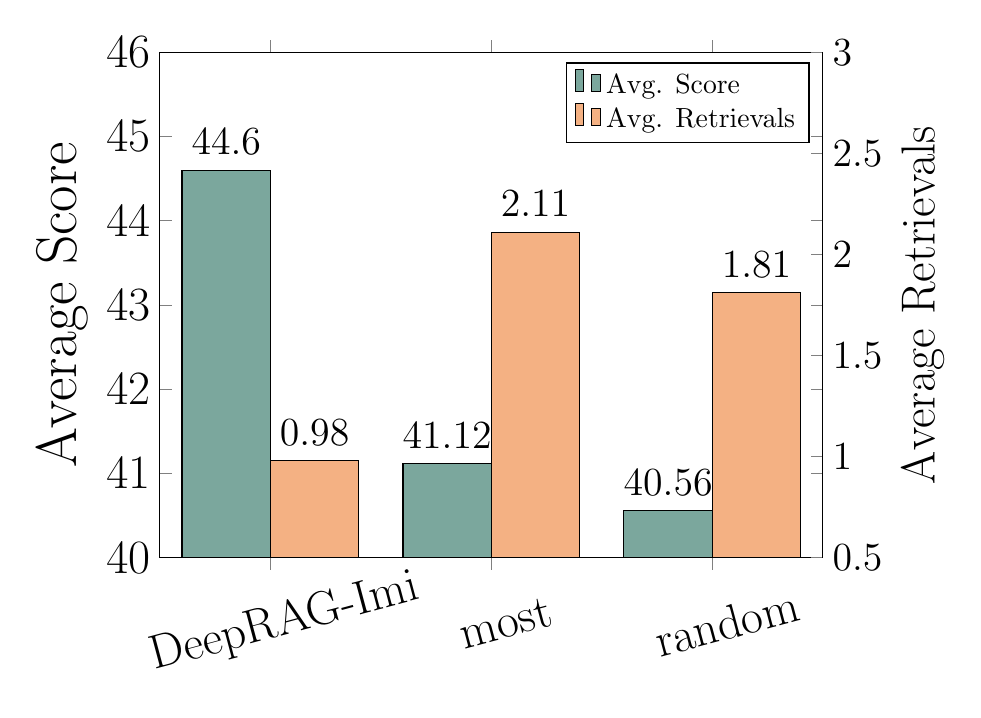
\begin{tikzpicture}
    \begin{axis}[
        width=10cm,
        height=8cm,
        ybar,
        xmin=0.5, xmax=3.5,
        ymin=40, ymax=46,
        xtick={1,2,3},
        xticklabels={DeepRAG-Imi,most,random},
        ticklabel style={font=\LARGE},
        xticklabel style={
            rotate=15,
            anchor=center,     % 让旋转后的文字对齐方式合理
            yshift=-20
          },
        label style={font=\LARGE},
        ylabel={Average Score},
        ylabel style={font=\huge},
        bar width=0.4,
        legend style={
            % at={(0.5,1.15)},    % 调整图例位置到图表上方
            anchor=north east,       % 设置锚点为北
            font=\normalsize,
            cells={anchor=west},
        }
    ]

    \addplot[
        fill={rgb,255:red,123; green,167; blue,157},
        nodes near coords,
        point meta=y,
        every node near coord/.append style={font=\Large, yshift=2pt}
    ] coordinates {
        (0.8,44.60)
        (1.8,41.12)
        (2.8,40.56)
    };
    \addlegendentry{Avg. Score}

    % 在第一个坐标系中添加第二个图例
    \addlegendimage{fill={rgb,255:red,244; green,177; blue,131}}
    \addlegendentry{Avg. Retrievals}

    \end{axis}

    \begin{axis}[
        width=10cm,
        height=8cm,
        ybar,
        xmin=0.5, xmax=3.5,
        ymin=0.5, ymax=3,
        axis x line=none,
        axis y line*=right,
        ticklabel style={font=\Large},
        label style={font=\LARGE},
        ylabel={Average Retrievals},
        ylabel style={font=\LARGE},
        bar width=0.4,
    ]

    \addplot[
        fill={rgb,255:red,244; green,177; blue,131},
        nodes near coords,
        point meta=y,
        every node near coord/.append style={font=\Large, yshift=2pt}
    ] coordinates {
        (1.2,0.98)
        (2.2,2.11)
        (3.2,1.81)
    };

    \end{axis}
    \end{tikzpicture}
}
            % \includegraphics[width=\textwidth]{figure/ablation1.pdf}
            (a)
        \end{minipage}
        \hfill
        \begin{minipage}[b]{0.48\textwidth}
            \centering
            
    \resizebox{\textwidth}{!}{
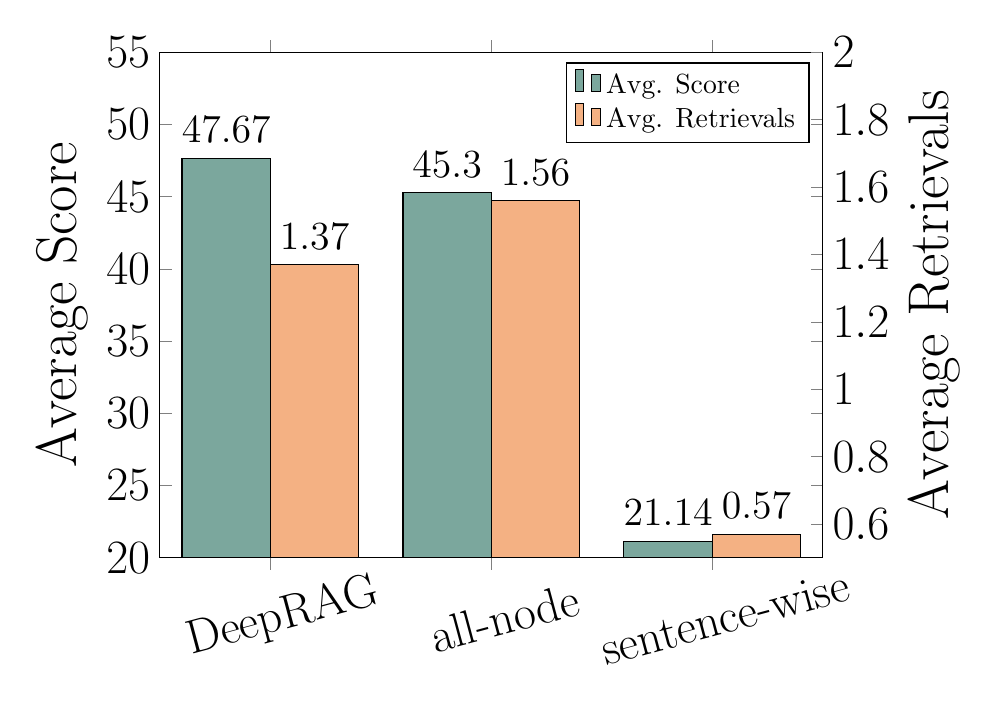
\begin{tikzpicture}

    %=======================%
    %   第一个 axis (左Y轴)
    %=======================%
    \begin{axis}[
        width=10cm,
        height=8cm,
        ybar,
        xmin=0.5, xmax=3.5,
        ymin=20, ymax=55,
        xtick={1,2,3},
        xticklabels={DeepRAG,all-node,sentence-wise},
        ticklabel style={font=\LARGE},     % 刻度字号
        xticklabel style={
            rotate=15,
            anchor=center,
            yshift=-18
        },
        label style={font=\Large},         % 轴标题字号
        ylabel={Average Score},
        ylabel style={font=\huge},
        bar width=0.4,
        legend style={
            % at={(0.5,1.15)},    % 调整图例位置到图表上方
            anchor=north east,       % 设置锚点为北
            font=\normalsize,
            cells={anchor=west},
        }
    ]

    %------ 左柱: Avg. Score ------%
    % 3 个方法, x=1-0.2=0.8, 2-0.2=1.8, 3-0.2=2.8
    \addplot[
        fill={rgb,255:red,123; green,167; blue,157},
        nodes near coords,
        point meta=y,
        every node near coord/.append style={font=\Large, yshift=2pt}
    ] coordinates {
        (0.8,47.67)
        (1.8,45.30)
        (2.8,21.14)
    };
    \addlegendentry{Avg. Score}

    % 为图例先添加一个条目(不用实际绘制), 代表右柱
    \addlegendimage{fill={rgb,255:red,244; green,177; blue,131}}
    \addlegendentry{Avg. Retrievals}

    \end{axis}

    %==========================%
    %   第二个 axis (右Y轴)
    %==========================%
    \begin{axis}[
        width=10cm,
        height=8cm,
        ybar,
        xmin=0.5, xmax=3.5,
        ymin=0.5, ymax=2.0,
        axis x line=none,
        axis y line*=right,
        ticklabel style={font=\LARGE},
        label style={font=\Large},
        ylabel={Average Retrievals},
        ylabel style={font=\huge},
        bar width=0.4,
    ]

    %------ 右柱: Avg. Retrievals ------%
    % x=1+0.2=1.2, 2+0.2=2.2, 3+0.2=3.2
    \addplot[
        fill={rgb,255:red,244; green,177; blue,131},
        nodes near coords,
        point meta=y,
        every node near coord/.append style={font=\Large, yshift=2pt}
    ] coordinates {
        (1.2,1.37)
        (2.2,1.56)
        (3.2,0.57)
    };

    \end{axis}

\end{tikzpicture}
}
            % \includegraphics[width=\textwidth]{figure/ablation2.pdf}
            (b)
        \end{minipage}
        \caption{Average score and retrievals on the ablation study for Imitation Learning and Chain of Calibration. }
        \label{fig:ablation}
    \end{minipage}
\end{figure*}





\paragraph{Imitation Learning}


\begin{table}[htbp]
  \centering
  \resizebox{\linewidth}{!}{
    \begin{tabular}{rccccc}
    \toprule
    Method & ID & CAG   & PopQA & WebQuestion & \multirow{2}[2]{*}{Avg} \\
             & F1    & EM    & EM    & EM    & \\
    \midrule
    \multicolumn{1}{l}{DeepRAG-Imi} &  \textbf{49.46}  & 50.47  & \textbf{43.60 } & \textbf{30.00 } & \textbf{44.60 } \\
    most & 47.31   & 51.09  & 31.30  & 28.00  & 41.12  \\
    random & 44.76   & \textbf{51.40 } & 34.80  & 27.10  & 40.56  \\
    \bottomrule
    \end{tabular}%
    }
    \caption{Experiment results of the ablation study on the Imitation Learning Stage. ID refers to the average score of two in-distribution dataset HotpotQA and 2WikiMultihopQA.}
  \label{tab:sft-abla}%
\end{table}%


We compare our default strategy of selecting paths with minimal retrieval cost against two alternative approaches: maximum retrieval cost and random path selection.
% 
As shown in Table~\ref{tab:sft-abla}, DeepRAG-Imi enables the model to learn knowledge boundaries during the imitation learning stage. 
Notably, CAG performs relatively poorly at this stage due to its time-sensitive nature, which necessitates constant retrieval of up-to-date information. 
% 
Moreover, as illustrated in Figure~\ref{fig:ablation}(a), DeepRAG-Imi achieves lower retrieval costs and higher average performance compared to both the maximum-retrieval-cost and random selection methods.





% Then, we analyze the impact of different methods for constructing pairs for chain of calibration. Speicifically, 相比于基于最优路径中的每个node构建偏好,我们比较了两种不同的构建策略,一种是对于所有node都构建pair,另一种是构建句子级别的偏序对。
% The ablation results of the chain of calibration process are shown in Table~\ref{tab:dpo-abla}. We observe that DeepRAG 想比另外两种变体有非常好的优势,特别地,从Figure 2(b)可以看出,DeepRAG可以achieve更低检索开销和更高的平均性能。而句子级别的偏序对学习到了不正确的偏好,过度依赖于内部知识导致了低检索开销和低性能。




% Table generated by Excel2LaTeX from sheet 'abaltion'
\begin{table}[t]
  \centering
  \resizebox{\linewidth}{!}{
    \begin{tabular}{rccccc}
    \toprule
    Method & ID & CAG   & PopQA & WebQuestion & \multirow{2}[2]{*}{Avg}\\
        & F1    & EM    & EM    & EM    &  \\
    \midrule
    \multicolumn{1}{l}{DeepRAG} & \textbf{52.40} & \textbf{61.92 } & \textbf{47.80 } & \textbf{45.24 } & \textbf{47.67 } \\
    all-node & 50.92   & 50.47  & 41.50  & 32.70  & 45.30  \\
    sentence-wise & 30.16   & 12.46  & 20.00  & 12.90  & 21.14 \\
    \bottomrule
    \end{tabular}%
    }
  \caption{Experiment results of the ablation study on the Chain of Calibration Stage.}
  \label{tab:dpo-abla}%
\end{table}%


\paragraph{Chain of Calibration} We compare our default approach of constructing preferences based on nodes from optimal paths against two alternatives: constructing pairs for all nodes and constructing sentence-level partial order pairs based on retrieval efficiency.
% 
As shown in Table~\ref{tab:dpo-abla}, DeepRAG demonstrates significant advantages over both variants. Specifically, as illustrated in Figure~\ref{fig:ablation}(b), DeepRAG achieves lower retrieval costs while maintaining higher average performance. In contrast, the sentence-level partial order pairs learned incorrect preferences, resulting in over-reliance on internal knowledge and consequently leading to both low retrieval costs and poor performance.


\begin{figure*}[htbp]
    \centering
    \includegraphics[width=1.0\linewidth]{figure/case.pdf}
    \caption{Case Study: Auto-RAG vs. DeepRAG. DeepRAG achieves success by atomic query decomposition, faithful intermediate answer, and adaptively using internal knowledge.}
    \label{fig:case-study}
\end{figure*}

\subsection{Performance against Strong Baseline Models}

% % In this section, we compare our DeepRAG with 最近一些较强的模型进行比较。
% % Specifically, we select the open-source o1-like model QwQ-32B~\cite{} and gpt-4o-turbo~\cite{}.
% As shown in Figure~\ref{tab:strong}, 通过基于dynamic cognitive decision 来利用external knowledge base, DeepRAG 在平均分 可以achieve 超过QwQ,尤其是在time-sensitve  QA表明DeepRAG不仅能够有效的认识到自我知识边界,还能适应time- sensitive场景。

In this section, we compare DeepRAG with recent strong baseline models. Specifically, we select two state-of-the-art open-source models: QwQ-32B-preview~\cite{qwq-32b-preview} and gpt-4o-turbo~\cite{OpenAI_hello_gpt4o}. 
% 
As shown in Table~\ref{tab:strong}, by leveraging external knowledge bases through dynamic cognitive decision-making, DeepRAG achieves superior average performance over QwQ and gpt-4o, particularly in time-sensitive QA tasks. 
% 
Notably, while DeepRAG does not surpass gpt-4o in some cases, it achieves comparable performance levels. 
% 
These results demonstrate that DeepRAG not only effectively recognizes its knowledge boundaries but also adapts well to time-sensitive scenarios.

% % Table generated by Excel2LaTeX from sheet 'final-latex'
% \begin{table}[htbp]
%   \centering
%   \resizebox{\linewidth}{!}{
%     \begin{tabular}{ccccccc}
%     \toprule
%     \multirow{2}[2]{*}{Models} & Hotpot QA & 2WMQA & CAG   & PopQA & WQ    & \multirow{2}[2]{*}{Avg} \\
%           & F1    & F1    & EM    & EM    & EM    &  \\
%     \midrule
%     QwQ-32B & 33.13  & 29.73  & 3.43  & 10.60  & 15.10  & 18.40  \\
%     gpt-4o-turbo & \textbf{58.81}  & \textbf{62.39}  & 23.36  & 43.50  & 25.35  & 42.68  \\
%     DeepRAG-qwen & 41.14  & 44.87  & 51.09  & 40.60  & 24.20  & 40.38  \\
%     DeepRAG-llama & 51.54  & 53.25  & \textbf{52.96}  & \textbf{42.50}  & \textbf{32.70}  & \textbf{46.59}  \\
%     \bottomrule
%     \end{tabular}%
%     }
%     \caption{Performance against strong baseline models.}
%   \label{tab:strong}%
% \end{table}%


% Table generated by Excel2LaTeX from sheet 'final-latex'
\begin{table}[htbp]
  \centering
  \resizebox{\linewidth}{!}{
    \begin{tabular}{cccccc}
    \toprule
    \multirow{2}[2]{*}{Models} & ID & CAG   & PopQA & WQ    & \multirow{2}[2]{*}{Avg} \\
          & F1      & EM    & EM    & EM    &  \\
    \midrule
    QwQ-32B & 31.43  & 3.43  & 10.60  & 15.10  & 18.40  \\
    gpt-4o-turbo & \textbf{60.6}  & 23.36  & 43.50  & 25.35  & 42.68  \\
    DeepRAG-qwen & 43.00  & 51.09  & 40.60  & 24.20  & 40.38  \\
    DeepRAG-llama & 52.40  & \textbf{52.96}  & \textbf{42.50}  & \textbf{32.70}  & \textbf{46.59}  \\
    \bottomrule
    \end{tabular}%
    }
    \caption{Performance against strong baseline models.}
  \label{tab:strong}%
\end{table}%



\subsection{Case Study}

As illustrated in Figure~\ref{fig:case-study}, we conduct a case study comparing DeepRAG with Auto-RAG~\cite{yu2024autorag}, a closely related method that utilizes iterative retrieval for retrieval-augmented generation.
% 
For each subquery, Auto-RAG retrieves relevant documents and generates a corresponding subanswer. This approach is not only time-consuming but also fails when no relevant documents are retrieved.
Although Auto-RAG attempts to address this issue using its own relevant documents, it falls into endless loops in most cases.
% 
In contrast, DeepRAG iteratively generates subqueries and determines whether to use internal knowledge at each iteration. The binary tree search data synthesis method for optimization ensures reliable subquery generation, intermediate answers, and final answers. Even when no related information exists in retrieved documents, the model is directed to provide a final answer based on internal knowledge.


% \subsection{Case study}
% % In Table~\ref{tab:casestudy}, we show a 典型的 case that 展示了SRAG的整个学习过程。In 对于问题“Where is the company that Sachin Warrier worked for as a software engineer headquartered”。 在stage1,SRAG 会首先obtain knowledge that Sachin Warrier worked for Tata Consultancy Services. Then, it 搜索 the headquarters of Tata Consultancy Services 从而获得答案是mumbai。而对于stage2, SRAG在检索到Sachin Warrier worked for Tata Consultancy Services之后,它利用内部知识回答了Tata Consultancy Services的首都在Mumbai。

% Table~\ref{tab:casestudy} provides a representative case study demonstrating the complete learning process of SRAG. For the query, ``Where is the company that Sachin Warrier worked for as a software engineer headquartered?'', SRAG follows distinct approaches in each stage. In Stage 1, the model initially acquires the knowledge that Sachin Warrier was employed at Tata Consultancy Services. Subsequently, it conducts a search to locate the headquarters of Tata Consultancy Services, retrieving the answer Mumbai. In Stage 2, however, after identifying that Sachin Warrier worked for Tata Consultancy Services, SRAG leverages its internal knowledge base to directly determine that the company's headquarters is in Mumbai, bypassing the need for an external search.